\chapter{Methodology}

Start with your overall approach to the research. What research problem or question did you investigate? What type of data did you need to answer it? Quantitative, qualitative, or mixed? Primary or secondary? Experimental or descriptive?
Describe the specific methods you used for data collection and analysis. How did you collect and analyze your data? What tools or materials did you use? How did you ensure the quality and accuracy of your data?
Explain why you chose these methods over others. How do they relate to your research question and literature review? How do they address the limitations or gaps in existing research? How do they suit your research design and objectives?
Evaluate and justify your methodological choices. How did they affect the outcome of your research? What challenges or difficulties did you encounter and how did you overcome them? How can you ensure the credibility and generalizability of your findings?

How this thesis is working?
Apparatus, Procedure, Utilities


\section{Android UI Data}
\subsection{Data tree structure}

\begin{figure}
    \centering
    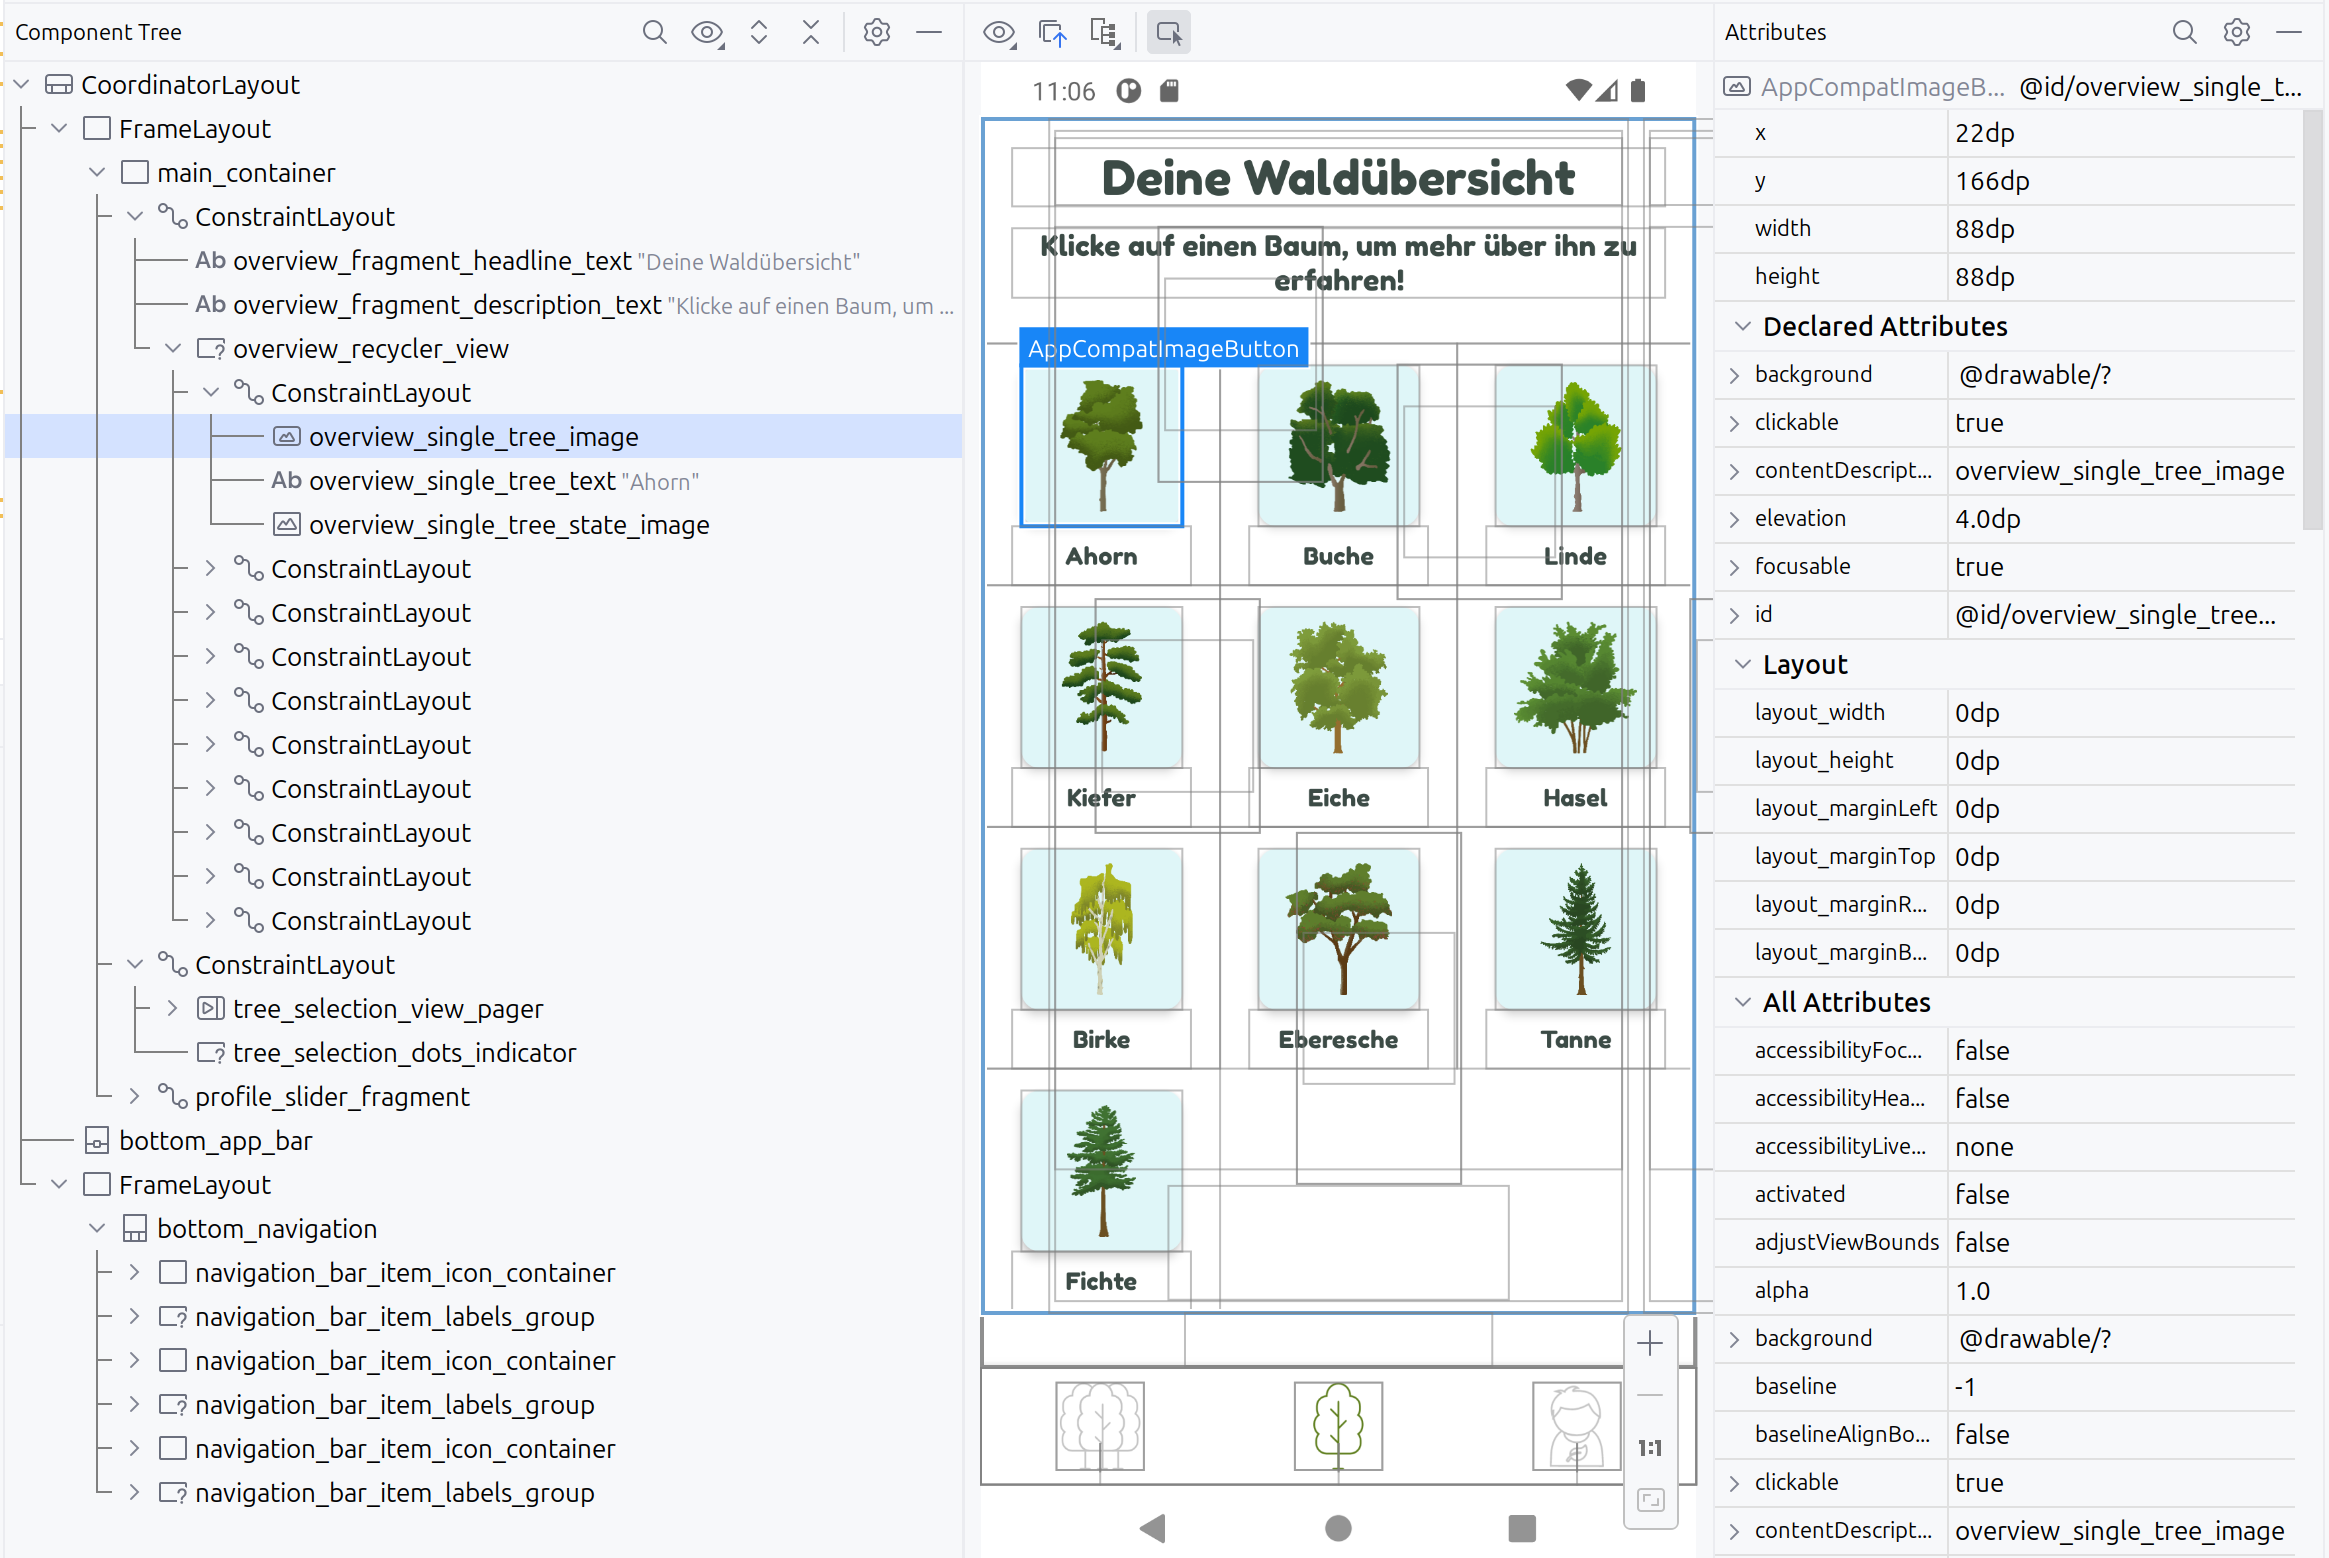
\includegraphics[width=\textwidth]{graphics/android_layout_inspector}
    \caption{https://developer.android.com/studio/debug/layout-inspector, https://github.com/mimuc/app-ins-gruene}
    \label{fig:android_layout_inspector}
\end{figure}

\subsection{Retrieval of UI data via Android Accessibility Service}

Semantics tree:
https://developer.android.com/jetpack/compose/semantics
https://android.googlesource.com/platform/frameworks/testing/+/jb-dev/uiautomator/library/src/com/android/uiautomator/core/AccessibilityNodeInfoDumper.java
https://github.com/Gustl22/android-accessibility/blob/c158808533d6fc017455184a7317555d3e6946f6/GlobalActionBarService/app/src/main/java/com/example/android/globalactionbarservice/uiautomator/AccessibilityNodeInfoDumper.java

\lstinputlisting[language=XML,label=android_accessibility_node,caption={Android Accessibility Node in XML.},float]{code/android_accessibility_node.xml}

\section{Machine Learning}
\subsection{Preprocessing}

Tensors, Datasets
%https://stackoverflow.com/a/48599383/5164462

\subsubsection{Feature selection}
Such as Filtering privacy invasive details

Parameterizing the vectorization process
a) Vector length
b) Weighting of features
c) Manipulating individual parameters of model

\subsubsection{Normalization}



\subsubsection{Padding}

\subsubsection{Embedding}

Category Embedding before LSTM
% https://stackoverflow.com/questions/47217151/keras-lstm-with-embedding-layer-before-lstm-layer
% https://stackoverflow.com/questions/52627739/how-to-merge-numerical-and-embedding-sequential-models-to-treat-categories-in-rn/52629902#comment136040845_52629902


- Embedding layer
Dimension near the actual average length of features (?)

\subsection{Supervised vs Unsupervised vs Semisupervised}
Reinforcement learning
\subsection{Under and Overfitting}
\subsection{Evaluation Metrics}
\section{Artificial Neural Nets}
Activation Functions
Cost function
Gradient
- Regression: Continous Values
- Classification: Multiple class
- One Class

\subsection{Classes of Neural Nets}

\subsubsection{Deep Neural Nets}
- Dense Layer

\subsubsection{Convolutional Neural Nets}
\subsubsection{Recurrent Neural Networks and LSTMs / GRU}
LSTM 4 dimensional
% https://stackoverflow.com/questions/54743549/is-it-possible-to-making-lstm-model-with-4-dimension-shape-of-data

Limitations to only 3 dimensions, needs flattening

Sample dimension (X -> y)
Time (Step) Dimension
Feature Dimension
Data, Quantity dimension, such as Image dimensions, or multiple nodes

TimeDistributedLayer
% https://stackoverflow.com/a/61588937/5164462
% https://stackoverflow.com/questions/53107126/what-are-the-uses-of-timedistributed-wrapper-for-lstm-or-any-other-layers

\subsubsection{Autoencoders}

Encoder, Decoder

\subsection{Tensorflow and Keras}
Layers
FlattenLayer

Positive Integer to Dense Vectors of fixed size

\section{Evaluation and Metrics}
\subsection{Mean Squared Error}
\subsection{F1 Score}
